\chapter{Implementation}

  In order to analyze how effective our attacks can steal links from graphs that are used to query inductive trained graph neural networks, we performed several experiments by attacking GNNs that have been trained to perform node classification.
  In this chapter we want to go through their implementation.
  We covered multiple datasets and types of graph neural network models, leading to an amount of \textasciitilde200 experiments.
  Due computational and time constraints, most of the parameters to optimize the attacks remain unexplored.

  \section{Datasets}

    For all our experiments, we used 3 datasets in total.
    In the table below, they are listed with their most interesting attributes.

    \vspace{0.48cm}
    \begin{table}[!h]
      \centering
      \footnotesize
      \begin{tabular}{l|l|l|l|l}
        \toprule
        Name & Number of Nodes & Number of Edges & Number of Classes & Feature Amount \\
        \midrule
        Cora & 2708            & 5429            & 7                 & 1433 \\
        CiteSeer & 3327        & 4732            & 6                 & 3703 \\
        Pubmed & 19717         & 44338           & 3                 & 500 \\
        \bottomrule
      \end{tabular}
      \caption{Dataset Information}
      \label{table:datasets}
    \end{table}

    \subsection*{Sample Datasets for Experiments}

      In order to fulfill the criteria that $G_s$ and $D_{f_t}$ are from the same dataset distribution like described in Section \refeq{section:threat-model}, we split our datasets and sample new ones based on our original three datasets \emph{Cora, CiteSeer} and \emph{Pubmed}.

      \subsubsection*{Same Dataset Distributions - Attack 1-2}
        Let $D = (V, E)$ be one of our three original datasets with $|V|$ nodes and $|E|$ edges.
        We can obtain two subgraphs by splitting $D$ into $D_{f_t} = (V_{f_t}, E_{f_t})$ and $D' = (V', E')$.
        We define $V_{f_t} = \{i$ | $\forall i \in V: random(0, 1) == 1\}$, where $random(0, 1)$ returns the values $0$ or $1$ at random, leading to a random split of the nodes, and $V' = \{j$ | $\forall j \in V: j \not\in V_{f_t}\}$.
        $D_{f_t}$ is used to train our target model $f_t$, while $D'$ is used to sample $G_{A}$, which is a graph, that was modified by deleting some known edges to simulate an incomplete graph.
        $D_A$ is obtained by querying $f_t$ on a subgraph of $G_A$. 

        \vspace{0.48cm}
        \begin{figure}[h!]
          \begin{center}
            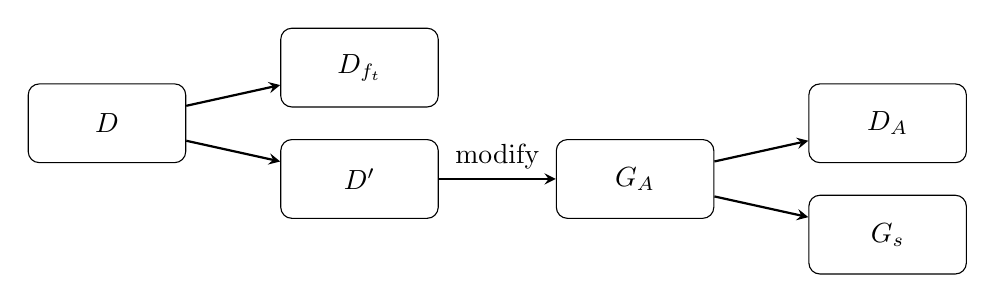
\begin{tikzpicture}
              
              % Definitions
              \tikzstyle{Dataset} = [rectangle, rounded corners,minimum width=2cm, minimum height=1cm, text centered, draw=black]
              \tikzstyle{arrow} = [thick,->,>=stealth]

              \node (D) [Dataset] {$D$};
              \node (Dft) [Dataset, above right of=D, xshift=2.5cm] {$D_{f_t}$};
              \node (D') [Dataset, below right of=D, xshift=2.5cm] {$D'$};
              \node (GA) [Dataset, right of=D', xshift=2.5cm] {$G_A$};
              \node (DA) [Dataset, above right of=GA, xshift=2.5cm] {$D_A$};
              \node (Gs) [Dataset, below right of=GA, xshift=2.5cm] {$G_s$};

              \draw [arrow] (D) -- node[anchor=south] {} (Dft);
              \draw [arrow] (D) -- node[anchor=south] {} (D');
              \draw [arrow] (D') -- node[anchor=south] {modify} (GA);
              \draw [arrow] (GA) -- node[anchor=south] {} (Gs);
              \draw [arrow] (GA) -- node[anchor=south] {} (DA);

              

            \end{tikzpicture}
          \end{center}
          \caption{Sampling Datasets - Same Dataset Distribution - Attack 1-2}
          \label{figure:sample-datasets-attack1-2}
        \end{figure}

        After $D$ has been split, we obtain $D' = (V', E')$ and define $G_A = (V_A, E_A)$ with $V_A = V'$ and $E_A = E'$.
        To sample $D_A$, we collect a set of positive samples $pos = \{(i,j, 1)$ | $\forall i,j \in V': (i,j) \in E' \wedge |pos| < ((1 - \alpha) * |E'|))\}$, containing pairs of nodes, that are connected in $D'$, where $\alpha$ denotes the percentage of known edges.
        Now, we collect a set of negative samples $neg = \{(i,j, 0)$ | $\forall i,j \in V': (i,j) \not\in E' \wedge |neg| < ((1 - \alpha) * |E'|))\}$, containing pairs of nodes, that are not connected in $D'$.
        We then delete all edges we sampled for $pos$, in our graph clone $G_A$, to simulate the missing edges, we want to steal.
        This leads to $E_A = \{(i,j)$ | $\forall (i,j) \in E': (i,j) \not\in pos\}$.
        $G_A$ is now a modified graph that contains less edges then the original graph $D'$ and we define a raw-dataset $raw = pos \cup neg$, containing the positive and negative samples obtained from $D'$.
        As the next step, we create the adversary's dataset $D_A = \{(post_{ij}, l)$ | $\forall (i,j,l)\in raw: post_{ij} = concat(f_t(G_A, i), f_t(G_A, j))\}$ for \emph{Attack 1} and $D_A = \{(dist_{ij}, l)$ | $\forall (i,j,l)\in raw: dist_{ij} = dist(post_i, post_j)\}$ for \emph{Attack 2}.
        $f_t(G_A, i)$ returns the node classification output posterior of the target model, when it is queried on $i$ given the adversary's graph $G_A$.
        $concat(a, b)$ concatenates the output posteriors $a$ and $b$ with each other returning the feature we will train the attacker model on.
        $l$ denotes the label either being 1 (positive sample) or 0 (negative sample).
        $dist(a,b) = [Cosine(a,b), ..., Sqeuclidean(a,b)]$, return the vector containing 8 different distance values like described in Section \refeq{section:threat-model}.
        With our adversary's dataset $D_A$ we can now continue training our attacker model using either $post_{ij}$ or $dist_{ij}$ as input features and $l$ as class.
        $G_s$, which is a subgraph of $G_A$ is unknown by the adversary while training. Neither the edges nor the nodes are used to train the attacker model.

      \subsubsection*{Different Dataset Distributions - Attack 3}
        Let $D_1$ and $D_2$ be two of our three original datasets.
        $D_1$ is used to sample $D_{f_A}$ and $G_A$.
        $D_{f_A}$ is used to train the adversary GNN $f_A$, while $G_A$ is used to query $f_A$ to obtain $D_A$, which will be used to train our attacker model $A$.
        $D_2$ is used to sample $D_{f_t}$ and $G_s$.
        $D_{f_t}$ is used to train our target model $f_t$, while $G_s$ is the incomplete graph, the adversary wants to steal links from.

        \vspace{0.48cm}
        \begin{figure}[h!]
          \begin{center}
            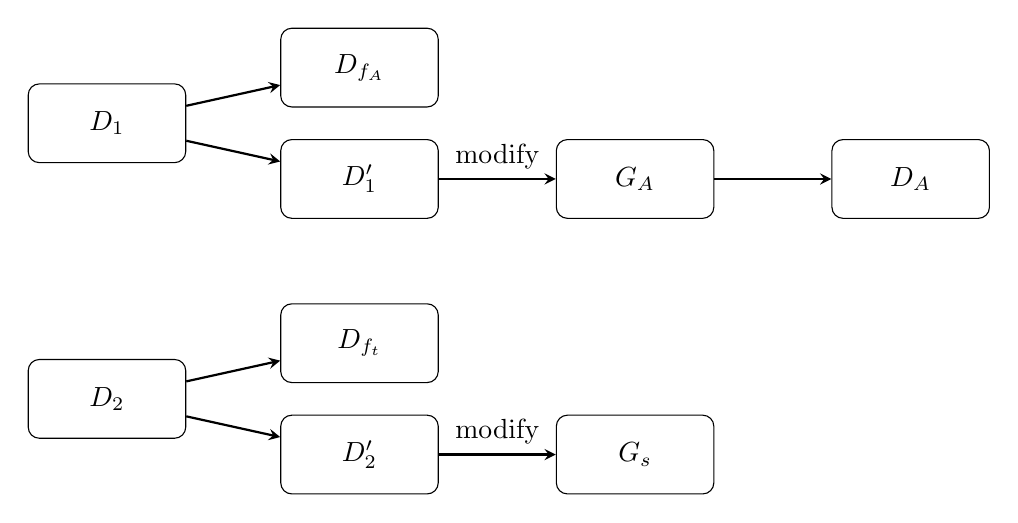
\begin{tikzpicture}
              
              % Definitions
              \tikzstyle{Dataset} = [rectangle, rounded corners,minimum width=2cm, minimum height=1cm, text centered, draw=black]
              \tikzstyle{arrow} = [thick,->,>=stealth]

              \node (D1) [Dataset] {$D_1$};
              \node (DfA) [Dataset, above right of= D1, xshift=2.5cm] {$D_{f_A}$};
              \node (D1') [Dataset, below right of= D1, xshift=2.5cm] {$D_1'$};
              \node (GA) [Dataset, right of= D1', xshift=2.5cm] {$G_A$};
              \node (DA) [Dataset, right of= GA, xshift=2.5cm] {$D_A$};


              \node (D2) [Dataset, below of =D1, yshift=-2.5cm] {$D_2$};
              \node (Dft) [Dataset, above right of= D2, xshift=2.5cm] {$D_{f_t}$};
              \node (D2') [Dataset, below right of= D2, xshift=2.5cm] {$D_2'$};
              \node (Gs) [Dataset, right of= D2', xshift=2.5cm] {$G_s$};
              
              \draw [arrow] (D1) -- node[anchor=south] {} (DfA);
              \draw [arrow] (D1) -- node[anchor=south] {} (D1');
              \draw [arrow] (D1') -- node[anchor=south] {modify} (GA);
              \draw [arrow] (GA) -- node[anchor=south] {} (DA);

              \draw [arrow] (D2) -- node[anchor=south] {} (Dft);
              \draw [arrow] (D2) -- node[anchor=south] {} (D2');
              \draw [arrow] (D2') -- node[anchor=south] {modify} (Gs);
              

            \end{tikzpicture}
          \end{center}
          \caption{Sampling Datasets - Different Dataset Distribution - Attack 3}
          \label{figure:sample-datasets-attack3}
        \end{figure}

        After $D_1$ has been split, we sample $D_A$ based on $D_1'$ the same way we did in \emph{Attack 1-2}.
        However, $G_s$ is considered to be from a different dataset distribution.
        That means, that we modify $D_2'$ the same way we modified $D_1'$, leading to a graph $G_s$ that contains less edges then the original one, simulating the links the adversary wants to steal. 
        Furthermore, like it was done in \emph{Attack 2}, we use $dist_{ij}$ as input for the attacker model instead of the posterior concatenation.


  \section{Target Models}

    As our target models, we used three different types of graph neural network models, each with a slightly different algorithm used to obtain the neighborhood embeddings.

    \subsection*{GraphSAGE}
      In June 2017 Hamilton et al.\cite{hamilton2018inductive} proposed a general framework, called GraphSAGE (SAmple and aggreGatE), for inductive node embedding. 
      They came up with an idea of leveraging node features like text attributes, node profile information or node degrees to learn an embedding function that generalizes to unseen nodes instead of prior approaches that use matrix factorization.
      Until then, the training process focused on individual embeddings for each node, but with the GraphSAGE algorithm, a function is learned that generates embeddings by sampling and aggregating features from a node's neighborhood.

    \subsection*{Graph Attention Networks}
      pass

    \subsection*{Graph Convolutional Networks}
      pass

    For each   


  \section{Attacker Model}
